\documentclass{beamer}
\usepackage[utf8]{inputenc}
\usetheme{Copenhagen}
\usepackage[spanish]{babel}
\usepackage{multirow}
%\usepackage{estilo-apuntes}
\usepackage{braids}
\usepackage[]{graphicx}
\usepackage{rotating}
\usepackage{pgf,tikz}
\usepackage{pgfplots}
\usepackage{tikz-cd}
\usetikzlibrary{arrows}
\usetikzlibrary{cd}
\usetikzlibrary{babel}
\pgfplotsset{compat=1.13}
\usetikzlibrary{decorations.shapes}
\pgfkeyssetvalue{/tikz/braid height}{1cm} %no parece hacer nada
\pgfkeyssetvalue{/tikz/braid width}{1cm}
\pgfkeyssetvalue{/tikz/braid start}{(0,0)}
\pgfkeyssetvalue{/tikz/braid colour}{black}

\theoremstyle{definition}

\newtheorem{teorema}{Theorem}
\newtheorem{defi}{Definition}
\newtheorem{prop}[teorema]{Proposition}

\newcommand{\Z}{\mathbb{Z}}
\newcommand{\C}{\mathbb{C}}
\newcommand{\CC}{\mathcal{C}}
\newcommand{\D}{\mathbb{D}}
\providecommand{\gene}[1]{\langle{#1}\rangle}


\addtobeamertemplate{navigation symbols}{}{%
    \usebeamerfont{footline}%
    \usebeamercolor[fg]{footline}%
    \hspace{1em}%
    %\insertframenumber/\inserttotalframenumber
}
\setbeamercolor{footline}{fg=black}
\setbeamerfont{footline}{series=\bfseries}

%-----------------------------------------------------------

\title{The Deligne Conjecture}
\author{Javier Aguilar Martín}
\institute{Universidad de Sevilla}
\date{}
 
\begin{document}
\frame{\titlepage}
%\begin{frame}
%
%c¡
%\title[About Beamer] %optional
%{About the Beamer class in presentation making}
% 
%\subtitle{A short story}
% 
%\author[Arthur, Doe] % (optional, for multiple authors)
%{A.~B.~Arthur\inst{1} \and J.~Doe\inst{2}}
% 
%\institute[VFU] % (optional)
%{
%  \inst{1}%
%  Faculty of Physics\\
%  Very Famous University
%  \and
%  \inst{2}%
%  Faculty of Chemistry\\
%  Very Famous University
%}

% 
%\date[VLC 2013] % (optional)
%{Very Large Conference, April 2013}


%\end{frame}
\setbeamercovered{highly dynamic}

\newcounter{saveenumi}
\newcommand{\seti}{\setcounter{saveenumi}{\value{enumi}}}
\newcommand{\conti}{\setcounter{enumi}{\value{saveenumi}}}

\resetcounteronoverlays{saveenumi}
%\AtBeginSection[]{
%\begin{frame}
%\frametitle{Tabla de contenidos}
%\tableofcontents
%\end{frame}
%}

%\begin{frame}
%	%AÑADIR ESTAS URL AL FINAL POR SI ME DA TIEMPO ENSEÑAR ESTAS COSAS 
%	%\url{https://www.blockchain.com/btc/blocks}
%	%\url{https://coin.dance/blocks}
%	%\url{https://www.blockchain.com/btc/unconfirmed-transactions}
%	
%%	ESTE TENGO PRIMERO QUE MIRARLO PARA HACERLO YO
%%	\url{https://anders.com/blockchain/}
%
%\end{frame}
\section{The Conjecture}
\begin{frame}
	\frametitle{Deligne Conjecture}
	\begin{block}{The conjecture}
	The action of the homology operad of little disks on the Hochschild cohomology of an associative algebra inducing its Gerstenhaber algebra structure lifts to an action of the chain operad of little disks on the Hochschild complex.
	\end{block}
	
\end{frame}

\begin{frame}
		\frametitle{Deligne Conjecture}
	\begin{block}{The conjecture}
	The action of the homology \textcolor{red}{operad} of little disks on the Hochschild cohomology of an associative algebra inducing its Gerstenhaber algebra structure lifts to an action of the chain operad of little disks on the Hochschild complex.
\end{block}
\end{frame}

\begin{frame}
	\frametitle{Deligne Conjecture}
	\begin{block}{The conjecture}
		The action of the \textcolor{red}{homology operad} of little disks on the Hochschild cohomology of an associative algebra inducing its Gerstenhaber algebra structure lifts to an action of the chain operad of little disks on the Hochschild complex.
	\end{block}
\end{frame}
\begin{frame}
	\frametitle{Deligne Conjecture}
	\begin{block}{The conjecture}
		The \textcolor{red}{action} of the \textcolor{red}{homology operad} of little disks on the Hochschild cohomology of an associative algebra inducing its Gerstenhaber algebra structure lifts to an action of the chain operad of little disks on the Hochschild complex.
	\end{block}
\end{frame}
\begin{frame}
		\frametitle{Deligne Conjecture}
	\begin{block}{The conjecture}
	The \textcolor{red}{action} of the \textcolor{red}{homology operad} of \textcolor{red}{little disks} on the Hochschild cohomology of an associative algebra inducing its Gerstenhaber algebra structure lifts to an action of the chain operad of little disks on the Hochschild complex.
\end{block}
\end{frame}

\begin{frame}
	\frametitle{Deligne Conjecture}
	\begin{block}{The conjecture}
		The \textcolor{red}{action} of the \textcolor{red}{homology operad} of \textcolor{red}{little disks} on the \textcolor{red}{Hochschild cohomology} of an associative algebra inducing its Gerstenhaber algebra structure lifts to an action of the chain operad of little disks on the Hochschild complex.
	\end{block}
\end{frame}

\begin{frame}
	\frametitle{Deligne Conjecture}
	\begin{block}{The conjecture}
		The \textcolor{red}{action} of the \textcolor{red}{homology operad} of \textcolor{red}{little disks} on the \textcolor{red}{Hochschild cohomology} of an associative algebra inducing its \textcolor{red}{Gerstenhaber algebra} structure lifts to an action of the chain operad of little disks on the Hochschild complex.
	\end{block}
\end{frame}

\begin{frame}
	\frametitle{Deligne Conjecture}
	\begin{block}{The conjecture}
		The \textcolor{red}{action} of the \textcolor{red}{homology operad} of \textcolor{red}{little disks} on the \textcolor{red}{Hochschild cohomology} of an associative algebra inducing its \textcolor{red}{Gerstenhaber algebra} structure lifts to an action of the \textcolor{green}{chain operad} of little disks on the Hochschild complex.
	\end{block}
\end{frame}

\begin{frame}
	\frametitle{Deligne Conjecture}
	\begin{block}{The conjecture}
		The \textcolor{red}{action} of the \textcolor{red}{homology operad} of \textcolor{red}{little disks} on the \textcolor{red}{Hochschild cohomology} of an associative algebra inducing its \textcolor{red}{Gerstenhaber algebra} structure lifts to an action of the \textcolor{green}{chain operad} of little disks on the \textcolor{green}{Hochschild complex}.
	\end{block}
\end{frame}



\begin{frame}
	\begin{itemize}
		\item Operads
		\begin{itemize}
			\item action of an operad (algebra over an operad)
			\item little disks operad
			\item chain/homology operad			
		\end{itemize}
	\item Gerstenhaber algebras
	\item Hochschild cohomology of an associative algebra
	\end{itemize}
\end{frame}

\section{Operads}

\begin{frame}
	\begin{itemize}
			\item<1-> An \textbf{operad} can be intuitively thought as a collection of spaces  $\CC=\{\CC(n)\}_{n\geq 0}$, whose points are thought to be $n$-ary operations $X^n\to X$. %decir que pueden ser (topological spaces, vector spaces, other objects) siempre que los axiomas tengan sentido, es decir, comentar que esto se puede hacer en cualquier categoría monoidal simétrica diciendo por encima lo que es: producto, unidad y axiomas. Poner algo de todos modos en alguna diapositiva
			\item<2-> We represent $n$-ary operations as trees with the following shape
			\begin{tikzpicture}[line cap=round,line join=round,>=triangle 45,x=1.0cm,y=1.0cm]
			\clip(-2.13333333333334,-0.093333333333332) rectangle (12.006666666666668,3.5);
			\draw [line width=2.pt] (2.,0.)-- (2.,1.);
			\draw [line width=2.pt] (2.,1.)-- (0.3666666666666659,3.);
			\draw [line width=2.pt] (2.,1.)-- (1.,3.);
			\draw [line width=2.pt] (2.,1.)-- (1.7,3.);
			\draw [line width=2.pt] (2.,1.)-- (3.,3.);
			\draw (0.1,3.493333333333331) node[anchor=north west] {$1$};
			\draw (0.8,3.52) node[anchor=north west] {$2$};
			\draw (1.5,3.493333333333331) node[anchor=north west] {$3$};
			\draw (2.8,3.453333333333331) node[anchor=north west] {$n$};
			\draw (2.1,3.453333333333331) node[anchor=north west] {$\cdots$};
			\end{tikzpicture}
	\end{itemize}

%\only<2->{\begin{defi}
%		An \textbf{operad} $\CC$ consists of topological spaces $\CC(j)$ for $j\geq 0$, together with the following data:
%		
%		\begin{itemize}
%			\item Continuous maps $\gamma : \CC(k) \times \CC(j_1) \times \cdots \times \CC(j_k) \to \CC(\sum_s j_s)$ such that the
%			following associativity formula is satisfied for all $c\in \CC(k)$, $d_s \in \CC(j_s)$, and $e_t \in \CC(i_t)$:
%			
%			\[\gamma(
%			\gamma(c; d_1, \dots , d_k); e_1, \dots , e_j) = 
%			\gamma(c; f_1, \dots , f_k),
%			\]
%			where $$f_s = \gamma(d_s; e_{j_1+\cdots+j_{s-1}+1}, \dots , e_{j_1+\cdots+j_s} ).$$%, and $f_s = *$ if $j_s = 0$ 
%			These maps are usually called \emph{structure maps}.
%			
%			
%			%{1,2,...,j} se divide en bloques y se permuta ese conjunto 
%		\end{itemize}
%	\end{defi}}
\end{frame}

\begin{frame}
	DIBUJOS DE LOS AXIOMAS ESCRIBIENDO LA NOTACIÓN QUE SE USA 
	
	MENCIONAR LAS INSERCIONES DEFINIDAS COMO PONER MUCHOS 1 EN EL GAMMA
	
	TENGO QUE DECIR QUE HAY MORFISMOS DE OPERADS AUNQUE SEA SIMPLEMENTE DECIR QUE RESPETAN LA ESTRUCTURA
\end{frame}
\begin{frame}
	COMENTAR QUE ESTA DEFINICIÓN SE PUEDE HACER EN CUALQUIER CATEGORÍA MONOIDAL SIMÉTRICA, DICIENDO LOS COMPONENTES DE LA DEFINICIÓN Y QUIZÁ DESTACANDO ALGÚN AXIOMA
	
   PONER EJEMPLOS
\end{frame}
\subsection{Algebras over an operad}
\begin{frame}
	\frametitle{Endomorphism operad}
	%SI LA CATEGORÍA ES LO BASTANTE BUENA (CLOSED) TENEMOS LO SIGUIENTE, POR COMODIDAD LO DEFINIMOS EN ESTA CATEGORÍA
	\begin{defi}
		Let $V$ be a finite-dimensional vector space over a field $k$. Then the \textbf{endomorphism operad} $\xi_V = \{ \xi_V(n) \}_{n\geq 0}$ of $V$ consists of
		\begin{itemize}
			\item<1-> $\xi_V(n)=\hom(V^{\otimes n},V)
			$ the space of linear maps $V^{\otimes n} \to V$.
			\item<2-> composition $\gamma(f; g_1, \dots, g_n)= f(g_1\otimes\dots\otimes g_n)$
			\item<3-> identity $\eta: k \to \xi_V(1)$, $1 \mapsto \operatorname{Id}_V$,
			\item<4->  symmetric group action $\gamma (f; g_1, \dots, g_n) \cdot \sigma = f (g_{\sigma^{-1}(1)} \otimes \dots \otimes g_{\sigma^{-1}(n)})$,  $\sigma \in \Sigma_n$.
		\end{itemize}\pause
\only<5>{	If $\mathcal{C}$ is another operad, each operad morphism $\mathcal{C} \to \xi_V$ is called an \textbf{algebra over} $\mathcal{C}$.}
		 %(notice this is analogous to the fact that each ''R''-module structure on an abelian group ''M'' amounts to a ring homomorphism <math>R \to \operatorname{End}(M)</math>.)
	\end{defi}
\end{frame}

\subsection{Little disks operad}
\begin{frame}
	\frametitle{Little Disks Operad}

\begin{defi}
	Let $E_2(n)$ be the configuration space of $n$ disks $B(x_i,r_i)$ of center $x_i\in D^2$ and radius $r_i\in (0,1]$ inside the standard unit disk $D^2$. 
	
	\begin{itemize}
		\item<2-> We call each $B(x_i,r_i)$ \textbf{little disk}.
		\item<3-> $E_2(n)$ can be viewed as a subspace of $(D^2\times (0,1])^n$ whose points are of the form $((x_1,r_1),\dots, (x_n,r_n))$ satisfying certain restrictions. % namely, $r_i$ must be such that the disk $B(x_i,r_i)\subset D^2$ does not intersect any other disk $B(x_j,r_j)$ and fits inside $D^2$. 
		\item<4-> By convention, $E_2(0)=\{*\}$.
	\end{itemize}
	 
\end{defi}
\end{frame}

\begin{frame}
	\definecolor{xdxdff}{rgb}{0.49019607843137253,0.49019607843137253,1.}
	\begin{figure}[h!]
	\resizebox{10cm}{4.7cm}{%
		\begin{tikzpicture}[line cap=round,line join=round,>=triangle 45,x=1.0cm,y=1.0cm]
		\clip(-4,-3.4) rectangle (9.5,3.4);
		\draw [line width=2.pt,color=xdxdff,fill=xdxdff,fill opacity=0.10000000149011612] (2.,1.) circle (0.7823042886243178cm);
		\draw [line width=2.pt,color=xdxdff,fill=xdxdff,fill opacity=0.10000000149011612] (3.,-1.) circle (1.100727032465361cm);
		\draw [line width=2.pt,color=xdxdff,fill=xdxdff,fill opacity=0.10000000149011612] (4.48,1.46) circle (0.7496665925596522cm);
		\draw [line width=2.pt] (3.,0.) circle (3.1622776601683795cm);
		\draw [line width=2.pt] (2.,1.) circle (0.7823042886243178cm);
		\draw [line width=2.pt] (4.48,1.46) circle (0.7496665925596522cm);
		\draw [line width=2.pt] (3.,-1.) circle (1.100727032465361cm);
		\draw (1.84,1.3) node[anchor=north west] {$1$};
		\draw (4.32,1.7) node[anchor=north west] {$2$};
		\draw (2.8,-0.8) node[anchor=north west] {$3$};
		%\draw (-1.44,0.6) node[anchor=north west] {\LARGE{$c=$}};
		\end{tikzpicture}
	}
	\caption{A point of $ E_2(3)$.}
\end{figure}
\end{frame}

\begin{frame}[fragile]
	\frametitle{Operad of little disks}
	
	 We define for all positive integers $p$ and $q$ and  each $1\leq i\leq p$ the insertion maps 
$$	
\begin{tikzcd}[row sep=10]
E_2(p)\times E_2(q)\arrow[r, "\circ_i"] & E_2(p+q-1)\\
(c_1,c_2)\arrow[r, mapsto, shorten <= 1em, shorten >= 1em] & c_1\circ_i c_2
\end{tikzcd}
$$

 \begin{figure}[h!]
	\centering
	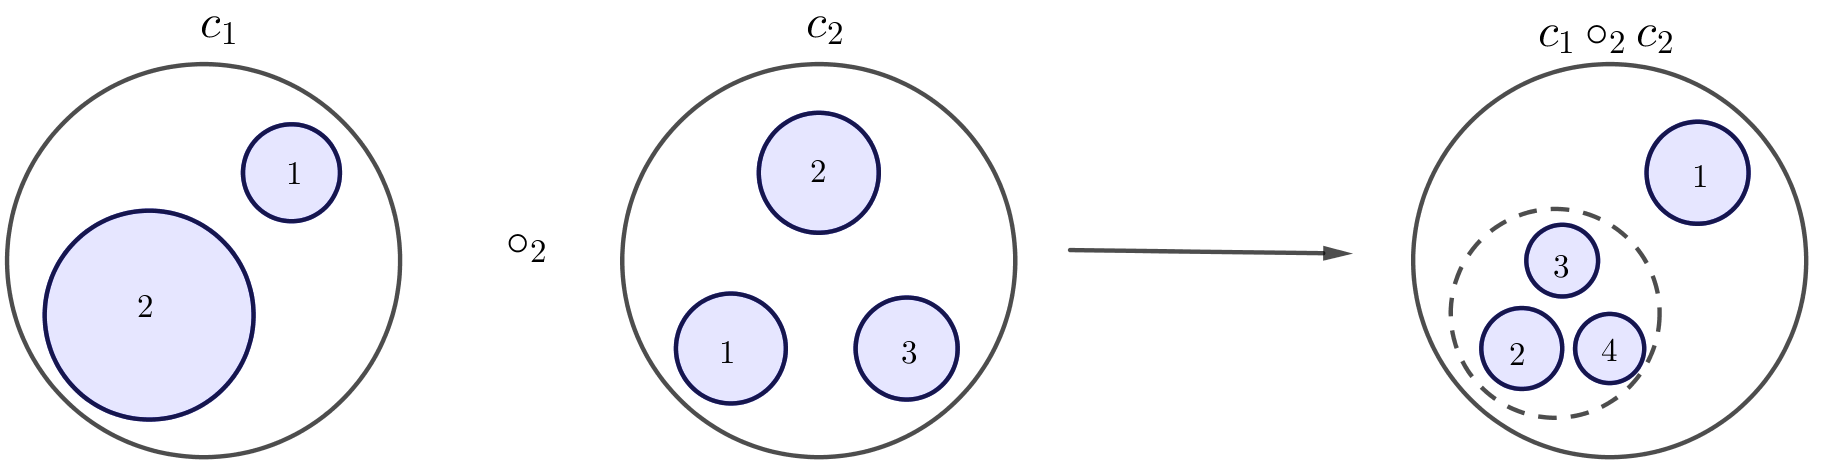
\includegraphics[scale=0.2]{Imagenes/insertion}
	\caption{An insertion $\circ_2:E_2(3)\times E_2(3)\to E_2(5)$.}
\end{figure}
	
\end{frame}

\begin{frame}
	\frametitle{Operad of little disks}
	IDENTIDAD: UN CÍRCULO CON EL 1 DENTRO
\end{frame}
\begin{frame}
	\frametitle{Operad of little disks}
	\begin{figure}[h!]
		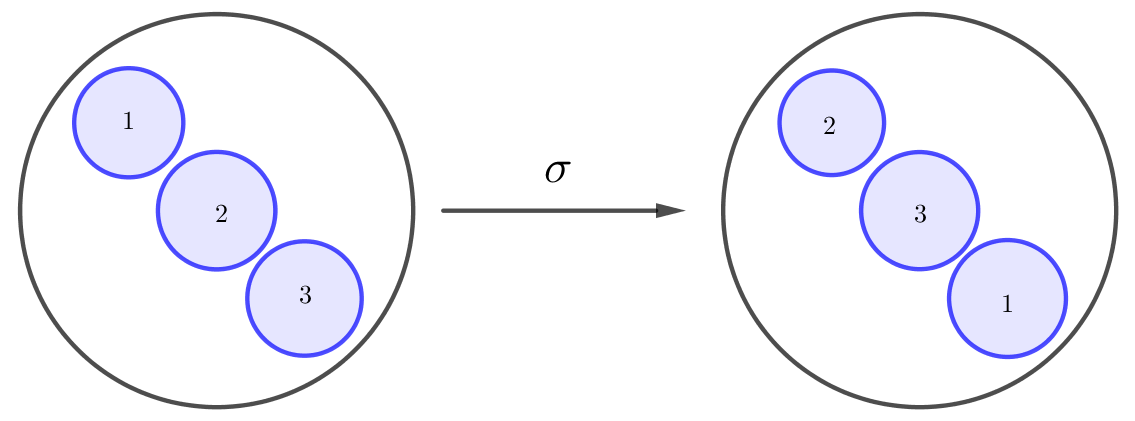
\includegraphics[scale=0.35]{Imagenes//accion}
		\caption{Action of $\sigma=(231)$ on a point of $E_2(3)$.}
	\end{figure}
\end{frame}


\section{Gerstenhaber algebras}

\begin{frame}
	\frametitle{Gerstenhaber algebras}
\end{frame}


\section{Hochschild cohomology of an associative algebra}

%\begin{frame}
%	\begin{block}{}
%	\begin{itemize}
%	\item An identity element $1 \in \CC(1)$ such that 
%	$\gamma(1; d) = d$ for $d \in \CC(j)$ and 
%	$\gamma(c; 1,\dots,1) = c$ for
%	$c \in \CC(k)$.
%	
%	\item A right action of the symmetric group $\Sigma_j$ on $\CC(j)$ such that the following equivariance
%	formulas are satisfied for all $c\in \CC(k)$, $d_s \in \CC(j_s)$, $\sigma\in\Sigma_k$, and $\tau_s\in\Sigma_{j_s}$:
%	\[
%	\gamma(c\sigma; d_1, \dots , d_k) = 
%	\gamma(c; d_{\sigma^{-1}(1)}, \dots , d_{\sigma^{-1}(k)})\sigma(j_1, \dots , j_k)
%	\]
%	and 
%	\[
%	\gamma(c; d_1\tau_1, \dots , d_k\tau_k) = \gamma(c; d_1, \dots , d_k)(\tau_1\oplus\cdots\oplus\tau_k),
%	\] 
%	where $\sigma(j_1, \dots , j_k)$ denotes the
%	permutation of $j$ letters which permutes the $k$ blocks of letters determined by the given
%	partition of $j$ (a first block of $j_1$, a second one of $j_2$ letters and so on), and $\tau_1\oplus\cdots\oplus\tau_k$ denotes the image of $(\tau_1, \dots , \tau_k)$ under the evident inclusion of $\Sigma_{j_1} \times \cdots \times \Sigma_{j_k}$ in $\Sigma_j$.
%\end{itemize}
%\end{block}
%
%\end{frame}


\begin{frame}
	Cada vez que explique una cosa ponerle un check a lo de antes \url{https://tex.stackexchange.com/questions/132783/how-to-write-checkmark-in-latex} (quizá en operads ponerlo al final al grande y ya)
\end{frame}

\begin{frame}
	Definición de operad y explicación dibujitos (más de los que he hecho en el trabajo)
	
	Operad de endomorfismos y álgebra sobre un operad
	
	Definición de operad en symmetric monoidal categories para que tenga sentido
	
	Comentar gracias al EZ map se hereda la operadición y de ahí a homología
	
	Las operaciones de la homología con los dos dibujitos (en el trabajo solo he metido uno)
	
	Gerstenhaber algebra definición del tirón (en la presentación comentar los criterios de derivación)
	
	Describir el complejo de cadenas sin detallar mucho en que es un complejo de cadenas e ir a su homología con sus propiedades de álgebra de Gerstenhaber (esto ya me relaciona con el último punto)
	
	Recuperar el homology operad y describir la acción sobre un álgebra asociativa
\end{frame}

\begin{frame}
	Retomar la conjetura de Deligne para recordarla y ver que está todo, seguido de un diagrama con las acciones y la que se pregunta si existe poniéndola dashed y con una interrogación de label
	
	Esquema de la prueba (destacar de algún modo las partes en las que me centro)
	
	Pensar qué meto de cada parte
\end{frame}

\end{document}
